\subsection{SAT $\propto$ 3--SAT}
\begin{enumerate}[(a)]
\item \begin{description}
\item[Énoncé de SAT] : \\
\begin{tabular}{r l l}
Données : & $ \mathcal{V} = \lbrace v_1, v_2 \ldots v_n \rbrace $ & \emph{Ensemble de $n$ variables}\\
& $ \mathcal{C} = \lbrace c_1, c_2, c_3 \ldots c_m \rbrace $ & \emph{Ensemble de $m$ clauses}\\
où & $ c_i = ( l_{i1} \vee l_{i2} \vee \cdots \vee l_{ik} ) $ & \emph{Clauses de $k$ littéraux}\\
avec & $ l_{ij} = v$ ou $ \neg v $ & \emph{avec $v \in U$} \\
\end{tabular}

Problème : existe-il au moins une affectation des variables telle que chaque clause de $\mathcal{C}$ soit vrai.

\item [Énoncé de 3--SAT] : 

3--SAT est identique au problème SAT avec $k = 3$.\\
\begin{tabular}{r l}
Données : & $ \mathcal{V} = \lbrace v_1, v_2, v_3 \ldots v_n \rbrace $\\
& $ \mathcal{C} = \lbrace c_1, c_2, c_3 \ldots c_m \rbrace $\\
où & $ c_i = ( l_{i1} \vee l_{i2} \vee l_{i3} ) $\\
avec & $ l_{ij} = v$ ou $ \neg v$\\
\end{tabular}
\end{description}
\item La réduction du problème SAT peut être définit en montrant que chaque clause $c$ de $\mathcal{C}$ peut-être transformée en un ensemble de clauses $\mathcal{C'}$ tel que pour toute affectation rendant vrai l'ensemble des clauses de $\mathcal{C}$, on peut trouver une affectation rendant vrai chaque clause de $\mathcal{C'}$. Chaque clause de $\mathcal{C'}$ devant être de taille exactement 3. La réciproque doit également être montrée.

Définissons les réductions :

\begin{description}
\item \mathversion{bold} $k = 1$ \mathversion{normal}

Soit $ci_1$ une clause de taille 1, on a $ci_1 = (l)$.
Ajoutons deux variables $v_1, v_2 \notin \mathcal{V}$ et transformons la clause $c$ en quatre clauses. On obtient l'ensemble $\mathcal{C}_1 = \lbrace c_1, c_2, c_3, c_4 \rbrace$ avec :
\[ c_1 = ( l \vee v_1 \vee v_2 )\]
\[ c_2 = ( l \vee v_1 \vee \neg v_2 )\]
\[ c_3 = ( l \vee \neg v_1 \vee v_2 )\]
\[ c_4 = ( l \vee \neg v_1 \vee \neg v_2 )\]

\item \mathversion{bold} $k = 2$ \mathversion{normal}

Soit $ci_2$ une clause de taille 2, on a $ci_2 = ( l_1 \vee l_2 )$.
Ajoutons une variable $v \notin \mathcal{V}$ et transformons la clause $c$ en deux clauses. On obtient l'ensemble $\mathcal{C}_2 = \lbrace c_1, c_2 \rbrace$ avec :
\[ c_1 = ( l_1 \vee l_2 \vee v )\]
\[ c_2 = ( l_1 \vee l_2 \vee \neg v )\]

\item \mathversion{bold} $k = 3$ \mathversion{normal}

La clause $ci_3$ ne subit pas de transformation.
\[ \mathcal{C}_3 = \lbrace ci_3 \rbrace \]

\item \mathversion{bold} $k > 3$ \mathversion{normal}

Soit la clause $ci_k = ( l_1 \vee l_2 \vee \cdots \vee l_k )$. On ajoute $(k - 3)$ nouvelles variables $(v_1, v_2 \ldots v_{k-3})$.

\[ \mathcal{C}_k = \underbrace{(l_1 \vee l_2 \vee v_1)}_{c_1} \bigwedge_{i=1}^{k-4}\left[ \underbrace{(\neg v_i \vee l_{i+2} \vee v_{i+1})}_{c_{i+1}}\right]  \wedge \underbrace{(\neg v_{k-3} \vee l_{k-1} \vee l_{k})}_{c_{k-2}} \]

Montrons que SAT est vrai si et seulement si 3--SAT est vrai :

\begin{description}
 \item \textbf{SAT $\rightarrow$ 3--SAT}
 
 	\begin{itemize}
 		\item Soit une interprétation $I_1$ qui satisfasse la clause $ci_1$ :
 		 \[ val(I_1,ci_1) = val(I_1,l) = vrai\]
 		
 		Prenons une interprétation $I_1'$ avec $val(I_1,l) = val(I_1',l)$, peu importe les affectations de $v_1$ et $v_2$, $l$ étant présent dans toutes les clauses de $\mathcal{C}_1$ :
 		\[ val(I_1',\mathcal{C}) = vrai \]
 		
 		\item Soit une interprétation $I_2$ qui satisfasse la clause $ci_2$ :
 		\[ \exists i, val(I_2,l_i) = vrai \]
 		Prenons une interprétation $I_2'$ avec :
 		\[ val(I_2,l_1) = val(I_2',l_1) \]
  		\[ val(I_2,l_2) = val(I_2',l_2) \]
  		Peu importe l'affectation de $v$ dans $I_2'$, on a $val(I_2',\mathcal{C}_2) = vrai$.
  		
  		\item Soit une interprétation $I_k$ qui satisfasse la clause $ci_k$ :
  		\[ \exists i, val(I_k,l_i) = vrai \]
  		
  		Prenons une interprétation $I_k'$ telle que :
  		\begin{eqnarray*}
  		val(I_k,l_i) & = & val(I_k',l_i)  \\
  		\forall j \in [1;(i-2)], val(I_k', v_j) & = & vrai \\
  		\forall j \in [(i-1);(k-3)], val(I_k', v_j) & = & faux \\
  		\end{eqnarray*}
  		
  		On obtient :
  		\[ val(I_k',\mathcal{C}_k) = vrai\]
  		
 	\end{itemize}
 	
 \item \textbf{3--SAT $\rightarrow$ SAT}
 
 	\begin{itemize}
 	\item Prenons une interprétation $I_1$ telle que $val(I_1,\mathcal{C}_1) = vrai$.
 	
 	Sans perte de généralité, on suppose que : 
 	\[ val(I_1,v_1) = val(I_1,v_2) = vrai \]
 	La clause $c_4$ de $\mathcal{C}_1$ ne peut être satisfaite que si $val(I_1,l) = vrai$.
 	
 	On a donc :
 	\[ val(I_1,ci_1) = vrai \]
 	
 	\item Prenons une interprétation $I_2$ telle que $val(I_2,\mathcal{C}_2) = vrai$.
 	
 	Sans perte de généralité on suppose que :
 	\[val(I_2,v) = vrai \]
 	
 	La clause $c_2$ de $\mathcal{C}_2$ ne peut être satisfaire que si $val(I_2,(l_1 \vee l_2)) = vrai$.
 	
 	On a donc :
 	\[ val(I_2,ci_2) = vrai \]
 	
 	\item Prenons une interprétation $I_k$ telle que $val(I_k,\mathcal{C}_k) = vrai$ et montrons qu'il existe forcément un $i$ tel que $val(I_k,l_i) = vrai$.
 	
 	Supposons que l'interprétation $I_k$ est modèle de $\mathcal{C}_k$ avec 
 	\[ \forall i \in [1;k], val(I_k,l_i) = faux \]
	\[ \Rightarrow val(I_k,v_1) = vrai  \textrm{ (dans $c_1$)} \]
	Donc :
	
	\begin{tabular}{lrl}
		& $\forall i \in [1;(k-4)], val(I_k,v_{i+1})$ & $= vrai$ \\
		$\Rightarrow$ & $val(I_k,v_{k-3})$ & $= vrai$ \\
		$\Rightarrow$ & $val(I_k,c_{k-2})$ & $= faux$ \\
		$\Rightarrow$ & $val(I_k,\mathcal{C}_k)$ & $= faux$
	\end{tabular}
	
	Pour que l'interprétation $I_k$ satisfasse $\mathcal{C}_k$, il doit exister un $i \in [1;k]$ tel que $val(I_k,l_i) = vrai$.
	
	On a donc :
	\[ val(I_k,ci_k) = vrai \]
 	 	
 	\end{itemize}
 
\end{description}

\end{description}

\item Le point (b) définit la réduction de SAT vers 3--SAT. Afin de montrer la NP-Complétude de 3--SAT, montrons que la réduction s’effectue en un temps polynomial.

Soit :
\begin{description}
\item $k$ la taille de la clause initiale,
\item $v_k$ le nombre de variables à ajouter pour obtenir des clauses de taille 3,
\item $w_k$ le nombre de clauses de taille 3 obtenues à partir de la clause initiale.
\end{description}
\begin{center}
\begin{tabular}{c c}
$v_3 = 0$ & $w_3 = 1$ \\
$v_4 = 1$ & $w_4 = 2$ \\
$v_5 = 2$ & $w_5 = 3$ \\
\vdots & \vdots
\end{tabular}
\end{center}

Pour tout $k > 3$ :
\[ v_k = v_{\left \lceil \frac{k}{2} \right \rceil + 1} + v_{\left \lfloor \frac{k}{2} \right \rfloor + 1} + 1 \]
\[ w_k = w_{\left \lceil \frac{k}{2} \right \rceil + 1} + w_{\left \lfloor \frac{k}{2} \right \rfloor + 1} \]

$v_k = \theta(k)$, donc borné par la taille de F. La réduction s'effectue donc en un temps polynomial.

Il est possible de réduire le problème SAT à 3--SAT en un temps polynomial, SAT étant NP-complet, 3--SAT l'est aussi.
\item Soit $\mathcal{C}$ un ensemble de clause à $n_v$ variables avec $n_1$ clauses de taille 1, $n_2$ clauses de taille 2, $n_3$ clauses de taille 3, $n_4$ clauses de taille 4 et $n_5$ clauses de taille 5. Calculons le nombre de variables et le nombre de clauses obtenues après réduction (respectivement $n_v'$ et $n_c'$).

Les points (b) et (c) permettent de déterminer pour une clause de taille $k$, le nombre de clause obtenues et le nombre de variables ajoutées après réduction. On peut donc en déduire la tableau suivant :

\begin{tabularx}{\textwidth}{| X || c | c | c | c | c |}
\hline
Taille de la clause dans $\mathcal{C}$	& 1 	& 2 	& 3 	& 4 	& 5 	\\
\hline
Nombre de clauses						& $n_1$	& $n_2$	& $n_3$	& $n_4$	& $n_5$	\\
\hline
Nombre de variables ajoutées par clause	& 2		& 1 	& 0 	& 1 	& 2 	\\
\hline
\textbf{Nombre de variables ajoutées au total} 	& $2n_1$& $n_2$	& 0		& $n_4$	& $2n_5$\\
\hline
Nombre de clauses obtenues par clause 	& 4 	& 2 	& 1 	& 2 	& 3 	\\
\hline
\textbf{Nombre de clauses obtenues au total}	& $4n_1$& $2n_2$& $n_3$	& $2n_4$& $3n_5$\\
\hline

\end{tabularx}

On a donc :
\[ n_v' = n_v + 2n_1 + n_2 + n_4 + 2n_5 \]
\[ n_c' = 4n_1 + 2n_2 + n_3 + 2n_4 + 3n_5 \]
\end{enumerate}

\subsection{3--SAT $\propto$ 2--SAT ?}
Cette réduction repose sur un principe qui consiste à décomposer une clause de taille $k$ en plusieurs clauses de tailles inférieures.

Soit une clause $c = (l_1 \vee l_2 \vee l_3)$ une clause de taille 3 et $I$ une interprétation qui satisfait $c$.

\begin{description}
\item[Cas 1 :] décomposons cette clause en deux clauses $c_1$ et $c_2$ de tailles 1 et 2 :
\begin{eqnarray*}
c_1&=&(l_1) \\
c_2&=&(l_2 \vee l_3)
\end{eqnarray*}
Pour montrer l'équivalence 3--SAT $\leftrightarrow$ 2--SAT, il faut ajouter une variable $v$ aux deux clauses créées :
\begin{eqnarray*}
c_1&=&(l_1 \vee v) \\
c_2&=&(l_2 \vee l_3 \vee \neg v)
\end{eqnarray*}

On a donc la clause $c_2$ de taille 3.

\item[Cas 2 :] décomposons cette clause en trois clauses $c_1$, $c_2$ et $c_3$ de taille 1 :
\begin{eqnarray*}
c_1 & = & (l_1) \\
c_2 & = & (l_2) \\
c_3 & = & (l_3)
\end{eqnarray*}

Pour montrer l'équivalence 3--SAT $\leftrightarrow$ 2--SAT, il faut ajouter deux variables $v_1$ et $v_2$ aux trois clauses créées :
\begin{eqnarray*}
c_1 & = & (l_1 \vee v_1 \vee \neg v_2) \\
c_2 & = & (l_2 \vee \neg v_1 \vee v_2)\\
c_3 & = & (l_3 \vee v_1 \vee v_2)
\end{eqnarray*}
On a donc également des clauses de taille 3. La réduction définie ci-avant ne permet donc pas la réduction de 3--SAT vers 2--SAT.
\end{description}




\subsection{2--SAT, un problème polynomial}
\begin{enumerate}[(a)]
\item Systèmes de deux clauses à deux littéraux :
\begin{description}
\item[Insatisfiable] : $(x \vee x) \wedge (\neg x \vee \neg x)$ \\
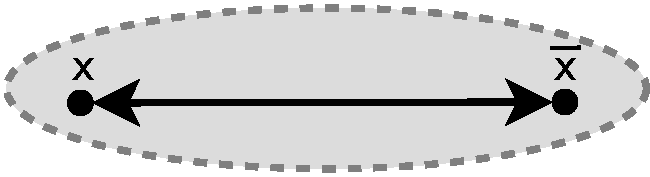
\includegraphics[width=5cm]{files/g1ex3.pdf}
\item[Valide] : $(x \vee \neg x) \wedge (x \vee \neg x)$ \\
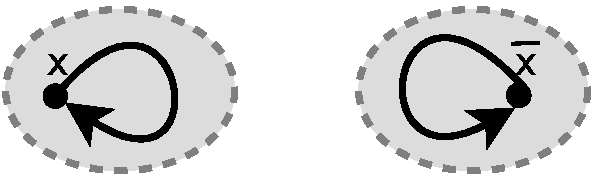
\includegraphics[width=5cm]{files/g2ex3.pdf}
\item[Contingent] : $(x \vee x) \wedge (x \vee x)$ \\
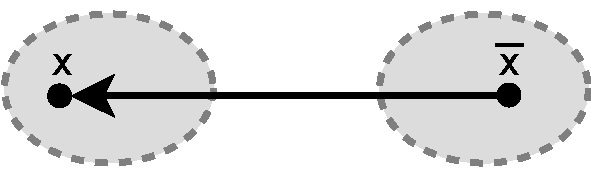
\includegraphics[width=5cm]{files/g3ex3.pdf}
\end{description}
\item 

L'insatisfiabilité du premier ensemble de clauses est clairement visible sur le graphe car les sommets $x$ et $\neg x$ sont dans la même composante fortement connexe.

Le deux autres ensembles sont satisfiables, les deux sommets ne sont pas dans la même composante fortement connexe.

\item L'algorithme suivant permet la génération du graphe correspondant à l'ensemble de clauses passé en paramètres.

\begin{algorithm}[H]
  \caption{GenererGraphe($\mathcal{C},\mathcal{V}$)}
  \Donnees{\\
  $\mathcal{C}$ \textit{// Ensemble de clauses}\\
  $\mathcal{V}$ \textit{// Ensemble des variables}
  }
  \Deb{
  Graphe.$\mathcal{S} = \emptyset$; \textit{// Ensemble des sommets du graphe}\\
  Graphe.$\mathcal{A} = \emptyset$; \textit{// Ensemble des arcs du graphe}\\
  \textit{// Initialisation des sommets}\\
  \PourTous{$v \in \mathcal{V}$}{
  ajouter(Graphe.$\mathcal{S}$,$v$)\;
  ajouter(Graphe.$\mathcal{S}$,$\neg v$)\;
  }
  \textit{// Parcours des clauses}\\
  \PourTous{$c \in \mathcal{C}$}{
  	ajouter(Graphe.$\mathcal{A}$,$(\neg c.x,c.y)$)\;
  	ajouter(Graphe.$\mathcal{A}$,$(\neg c.y,c.x)$)\;
  }
    \Retour Graphe\;
  }
\end{algorithm}
Cet algorithme effectue un parcours de $\mathcal{V}$ et un parcours de $\mathcal{C}$, sa complexité est donc $O(|\mathcal{C}|+|\mathcal{V}|)$.

\item Les composantes fortement connexes du graphe généré peuvent être calculées par l'algorithme de Tarjan.

\begin{algorithm}[H]
  \caption{Principale($G$)}
  \Donnees{
  $G$ \textit{// Le graphe}
  }
  \Deb{
  date\;
  \PourTous{$x \in G.\mathcal{S}$}{
  DEBUT[$x$] $\leftarrow 0$\;
  CFC[$x$] $\leftarrow 0$\;
  }
  Pile $\leftarrow \emptyset$\;
  numCFC $\leftarrow 0$\;
  
  \PourTous{$s \in G.\mathcal{S}$}{
  \Si{DEBUT[$s$] $= 0$}{
  Tarjan($s$,date,DEBUT,Pile,numCFC,CFC)\;
  }
  
  }
    \Retour Comp;
  }
\end{algorithm}

\begin{algorithm}[H]
  \caption{Tarjan($s$,date,DEBUT,Pile,numCFC,CFC)}
  \Donnees{\\
  s \textit{// Le sommet}\\
  date \textit{// Date de visite}\\
  DEBUT \textit{// Tableau de visites}\\
  Pile \textit{// Pile de sommets}\\
  numCFC \textit{// Numéro de la CFC}\\
  CFC \textit{// Liste des CFC}\\
  }
  \Deb{
	date $\leftarrow$ date$+1$\;
	DEBUT[$s$]=date\;
	min $\leftarrow$ DEBUT[$s$]\;
	Empiler(Pile,$s$)\;
	\PourTous{$j \in $Adj[$i$]}{
	\lSi{DEBUT[$j$]$=0$}{
	min $\leftarrow$ MIN(min,Tarjan($j$))\;
	}
	\lSinonSi{CFC[$j$]$=0$}{
	min $\leftarrow$ MIN(min,DEBUT[$j$])\;
	}
	}
	\Si{min$=$DEBUT[$i$]}{
	Ncfc $\leftarrow$ numCFC $+1$\;
	}
	\Repeter{$k \neq i$}{
	$k \leftarrow$ Depiler(Pile)\;
	CFC[$k$] $\leftarrow$ numCFC\;
	}
    \Retour Comp;
	}
  
\end{algorithm}

\end{enumerate}
